\documentclass{article}
\usepackage{graphicx}
\usepackage{amsmath}

\begin{document}
\section{Calculation Practice}

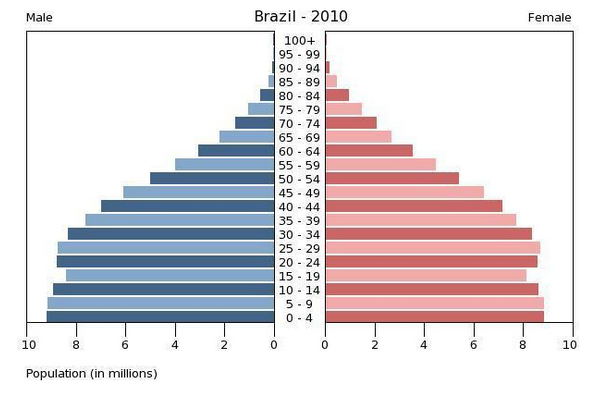
\includegraphics[width=\textwidth]{images/calculation-practice.png}

\subsection{If the population of Brazil was approximately 200 million in 2010, what was the percentage of pre-reproductive females?}

\begin{gather}
    \sum females\ age<15 \approx 26\ million \\
    \frac{26\ million\ pre\ reproductive\ females}{200\ million\ people} = 13\%
\end{gather}

\subsection{What is the approximate percentage of retirement age adults?}

\begin{gather}
    \sum adults\ age>64 \approx 18\ million \\
    \frac{18\ million\ retired\ adults}{200\ million\ people} = 9\%
\end{gather}

\subsection{If Brazil’s CBR is 16 and the CDR is 6, what is the doubling time?}

\begin{gather}
    r = \frac{16\ births - 6\ deaths}{1000\ people} = 1\% \\
    t = \frac{70}{r} = 70\ years
\end{gather}

\subsection{With this growth rate, what would the population be in 2011?}

\begin{gather}
    p_{2010} = 2 * 10^6\ people \\
    p_{2011} = p_{2010} * (1 + r) = 2.02 * 10^8\ people
\end{gather}

\subsection{If the population grew to 210 million over the next 6 years, on average, how many people would be added each year? }

\begin{gather}
    \overline{\delta /year} = \frac{\delta pop}{t} \\
    1.67 * 10^6\ people/year
\end{gather}

\end{document}


